
\documentclass{beamer}		% This tells LaTeX the document will be a "beamer" presentation

\mode<presentation>
{
  \usetheme{Madrid}      % or try Darmstadt, Madrid, Warsaw, ...
  \usecolortheme{default} % or try albatross, beaver, crane, ...
  \usefonttheme{serif}  % or try serif, structurebold, ...
  \setbeamertemplate{navigation symbols}{}
  \setbeamertemplate{caption}[numbered]
} 

\usepackage{amsmath}
\usepackage{amssymb}
\usepackage{amsfonts}
\usepackage{bm}
\usepackage{subfigure}
\usepackage{geometry}
\usepackage{graphicx}
\usepackage{graphbox}
\usepackage[backend=bibtex,sorting=none]{biblatex}

\addbibresource{references.bib}
\setbeamerfont{footnote}{size=\tiny}
\setbeamertemplate{bibliography item}[text]

\newcommand{\light}[1]{\textcolor{gray}{#1}}
\newcommand{\dd}{\mathrm{d}}
\newcommand{\R}{\mathbb{R}}
\newcommand{\E}{\mathbb{E}}

\DeclareMathOperator*{\argmax}{arg\,max}
\DeclareMathOperator*{\argmin}{arg\,min}
\DeclareMathOperator*{\KL}{KL}
\DeclareMathOperator*{\ELBO}{ELBO}

\title[Semi-Amortized Variational Autoencoders]{Semi-Amortized Variational Autoencoders}	% Insert your title.  Depending on the theme you choose above, a "short title" might be useful, as it will appear on the footer of each slide.

\author[Yoon Kim, Sam Wiseman, Andrew C. Miller, David Sontag and Alexander M. Rush ]{Yoon Kim, Sam Wiseman, Andrew C. Miller, David Sontag and Alexander M. Rush \\  presenter: Shen Yuan} % Insert your name

% \institute[UoE]{University of Edinburgh} % Self-explanatory



\begin{document} 	% Let's begin

% Presentations come in slide frames.  You have to tell LaTeX when to start a frame, and when to end the frame.  The most common error beginners make with beamer is forgetting the \end{frame} command.	


\begin{frame}	

\titlepage	% Prints a title page populated with the information given in the preamble
	
\end{frame}	


\begin{frame}[noframenumbering]
\begin{itemize}
    \begin{LARGE}
    \item Background
    \item \light{Semi-Amortized Variational Autoencoders}
    \item \light{Experiments}
    \end{LARGE}
\end{itemize}
\end{frame}



\begin{frame}{Background of Variational Inference}

Here is a unknown distribution $p(\bm{x};\theta)$, we need to calculate its parameters $\theta$.

\begin{figure}[t]
\centerline{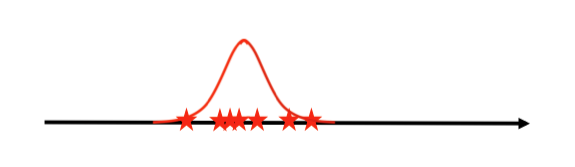
\includegraphics[width=0.7\linewidth]{figure1.png}}
\vspace{-10pt}
\label{fig1}
\end{figure}

\begin{itemize}
    \pause
    \item sample $\bm{x}=\{x_1, x_2, \ldots, x_n\}$ from the distribution
    \pause
    \item assume it is a gaussian distribution with $\theta = \{\mu, \sigma^2\}$
    \pause
    \item maxmize its likelihood function $\hat{\theta} = \argmax_{\theta} \hat{L}_n(\theta;\bm{x})$
\end{itemize}

\end{frame}



\begin{frame}{Probabilistic latent variable models}

However, what happens very often is we don't actually know whether the unknown distribution consists of many other hidden distributions.

\begin{figure}[t]
\centerline{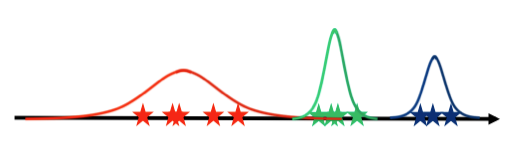
\includegraphics[width=0.7\linewidth]{figure2.png}}
\vspace{-10pt}
\label{fig1}
\end{figure}

\begin{figure}[t]
\centerline{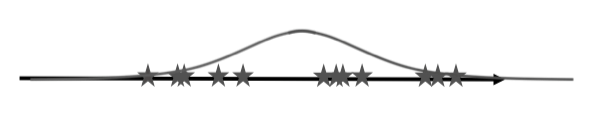
\includegraphics[width=0.7\linewidth]{figure3.png}}
\vspace{-10pt}
\label{fig1}
\end{figure}
    
\end{frame}



\begin{frame}{Probabilistic latent variable modelse}

That is why to introduce the latent variable $\bm{z} = \{z_1, z_2, \ldots, z_n\}$, which describes the probabilities of each sample generated by each hidden distribution.

\begin{eqnarray*}
\begin{aligned}
p(\bm{x};\theta) = \sum_{z\in\bm{z}} p(\bm{x}|z;\theta)p(z)  = \int p(\bm{x}|z;\theta)p(z)\dd z 
\end{aligned}    
\end{eqnarray*}

\begin{figure}[t]
\centerline{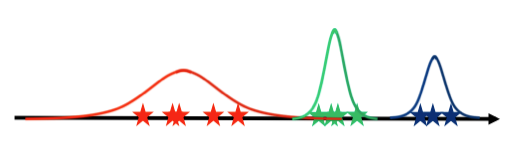
\includegraphics[width=0.7\linewidth]{figure2.png}}
\vspace{-10pt}
\label{fig1}
\end{figure}
    
\end{frame}



\begin{frame}{Probabilistic latent variable models}

\begin{itemize}
    \item sample $\bm{x} \sim p(\bm{x};\theta)$
    \item calculate $p(\bm{z}|\bm{x};\theta)$ based on $\bm{x}$
    \item calculate $p(\bm{x}|\bm{z};\theta)$ based on $\bm{z}$
    \item get $p(\bm{x};\theta)$
\end{itemize}

\pause
~\\
How to get $p(\bm{z}|\bm{x})$?

\end{frame}



\begin{frame}{Variational inference}

The goal of variational inference is to approximate a conditional density of latent variables by defining a variational family of distributions $q(\bm{z};\lambda)$ parameterized by $\lambda$.

\begin{eqnarray*}
\begin{aligned}
q_i(\bm{z};\lambda_i) \sim p(\bm{z}|\bm{x}_i)
\end{aligned}    
\end{eqnarray*}

For each sample $x_i$, there is a corresponding distribution $q_i$ to indicate which hidden distribution it belongs to.

\end{frame}



\begin{frame}{Variational inference}

\begin{small}
\begin{eqnarray*}
\begin{aligned}
\KL(q(\bm{z};\lambda)||p(\bm{z}|\bm{x})) &= \E_{\bm{z} \sim q(\bm{z};\lambda)}[\log(q(\bm{z};\lambda)) - \log(p(\bm{z}|\bm{x}))]\\
&= \E_{\bm{z} \sim q(\bm{z};\lambda)}[\log(q(\bm{z};\lambda)) - \log(\frac{p(\bm{x}|\bm{z})p(\bm{z})}{p(\bm{x})})]\\
&= \E_{\bm{z} \sim q(\bm{z};\lambda)}[\log(q(\bm{z};\lambda)) - \log(p(\bm{x}|\bm{z})) - \log(p(\bm{z}))] + \log(p(\bm{x}))\\
&= \E_{\bm{z} \sim q(\bm{z};\lambda)}[\log(\frac{q(\bm{z};\lambda)}{p(\bm{z})}) - \log(p(\bm{x}|\bm{z}))] + \log(p(\bm{x}))\\
&= \KL[q(\bm{z};\lambda)||p(\bm{z})] - \E_{\bm{z} \sim q(\bm{z};\lambda)}[log(p(\bm{x}|\bm{z}))] + \log(p(\bm{x}))\\
&= \log(p(\bm{x})) - \{\E_{\bm{z} \sim q(\bm{z};\lambda)}[\log(p(\bm{x}|\bm{z}))] - \KL[q(\bm{z};\lambda)||p(\bm{z})]\}\\
\pause
&= \log(p(\bm{x})) - \ELBO(\lambda, \theta, \bm{x})
\end{aligned}    
\end{eqnarray*}
\end{small}

\end{frame}



\begin{frame}{Stochastic Variational Inference}

\begin{itemize}
    \item sample $\bm{x}\sim p(\bm{x})$
    \item randomly initialize $\lambda_0, \theta$
    \item for $k=0,\ldots,K-1$, set \\ $\lambda_{k+1} = \lambda_k + \alpha \nabla_{\lambda} \ELBO(\lambda_k, \theta, \bm{x})$
    \item update $\theta$ based on $\nabla_{\theta} \ELBO(\lambda_k, \theta, \bm{x})$
\end{itemize}

\pause
~\\
This procedure, which is repeated for each example, is computationally expensive and requires setting step-size hyper-parameters $\alpha$.

\end{frame}



\begin{frame}{Amortized Variational Inference}

Amortized Variational Inference uses a shared parametric inference model(i.e., $\text{encoder}(\cdot)$) to predict the  parameters $\lambda_i$ for each example $x_i$.
The word 'Amortized' means a shared model.

~\\
\begin{itemize}
    \item sample $\bm{x}\sim p(\bm{x})$
    \item set $\lambda = \text{encoder}(\bm{x};\phi)$
    \item update $\theta$ based on $\nabla_{\theta} \ELBO(\lambda, \theta, \bm{x})$
    \item update $\phi$ based on $\nabla_{\phi} \ELBO(\lambda, \theta, \bm{x})$ \\ $\frac{\dd \ELBO(\lambda, \theta, \bm{x})}{\dd \phi} = \frac{\dd \lambda}{\dd \phi} \nabla_\lambda \ELBO(\lambda, \theta, \bm{x})$
\end{itemize}
    
\end{frame}



\begin{frame}[noframenumbering]
\begin{itemize}
    \begin{LARGE}
    \item \light{Background}
    \item Semi-Amortized Variational Autoencoders
    \item \light{Experiments}
    \end{LARGE}
\end{itemize}
\end{frame}



\begin{frame}{Semi-Amortized Variational Autoencoders}

However, requiring all the variational parameters $\bm{\lambda} = \{\lambda_1, \ldots, \lambda_n\}$ to be a parametric function of the input may be too strict of a restriction and can lead to an amortization gap.
    
\end{frame}



\begin{frame}{Semi-Amortized Variational Autoencoders}

\begin{itemize}
    \item sample $\bm{x}\sim p(\bm{x})$
    \item set $\lambda_0 = \text{encoder}(\bm{x};\phi)$
    \item for $k=0,\ldots,K-1$, set \\ $\lambda_{k+1} = \lambda_k + \alpha \nabla_{\lambda} \ELBO(\lambda_k, \theta, \bm{x})$
    \item update $\theta$ based on $\frac{\dd \ELBO(\lambda_K, \theta, \bm{x})}{\dd \theta}$
    \item update $\phi$ based on $\frac{\dd \ELBO(\lambda_K, \theta, \bm{x})}{\dd \phi}$
\end{itemize}

\end{frame}



\begin{frame}{Semi-Amortized Variational Autoencoders}

\begin{figure}[H]
\centering
\subfigure{
\label{Fig.sub.11}
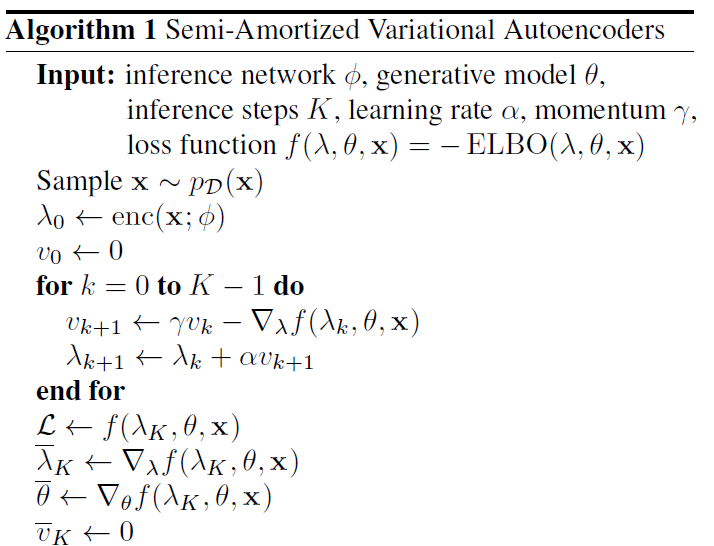
\includegraphics[width=0.45\textwidth]{figure4.png}}
\subfigure{
\label{Fig.sub.12}
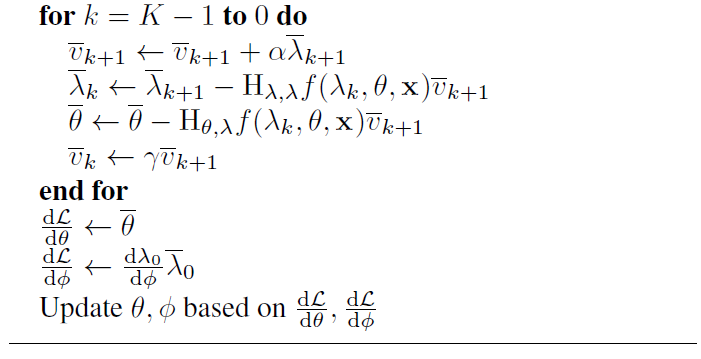
\includegraphics[width=0.45\textwidth]{figure5.png}}
\label{fig1}
\end{figure}

\end{frame}



\begin{frame}{Semi-Amortized Variational Autoencoders}

This paper calculated Hessian-vector products with finite differences, which was found to be more memory-efficient than automatic differentiation.

\begin{eqnarray*}
\begin{aligned}
H_{\bm{u}_i,\bm{u}_j}f(\hat{u})\bm{v} \approx \frac{1}{\epsilon} ( &\nabla_{\bm{u}_i}f(\hat{\bm{u}}_0,\ldots,\hat{\bm{u}}_j+\epsilon \bm{v}, \ldots, \hat{\bm{u}}_m)\\
&- \nabla_{\bm{u}_i} f(\hat{\bm{u}}_0,\ldots,\hat{\bm{u}}_j,\ldots,\hat{\bm{u}}_m ) )
\end{aligned}    
\end{eqnarray*}

where $\epsilon$ is some small number (we use $\epsilon = 10^{-5}$).

\end{frame}



\begin{frame}[noframenumbering]
\begin{itemize}
    \begin{LARGE}
    \item \light{Background}
    \item \light{Semi-Amortized Variational Autoencoders}
    \item Experiments
    \end{LARGE}
\end{itemize}
\end{frame}



\begin{frame}{Experiments}

\begin{figure}[t]
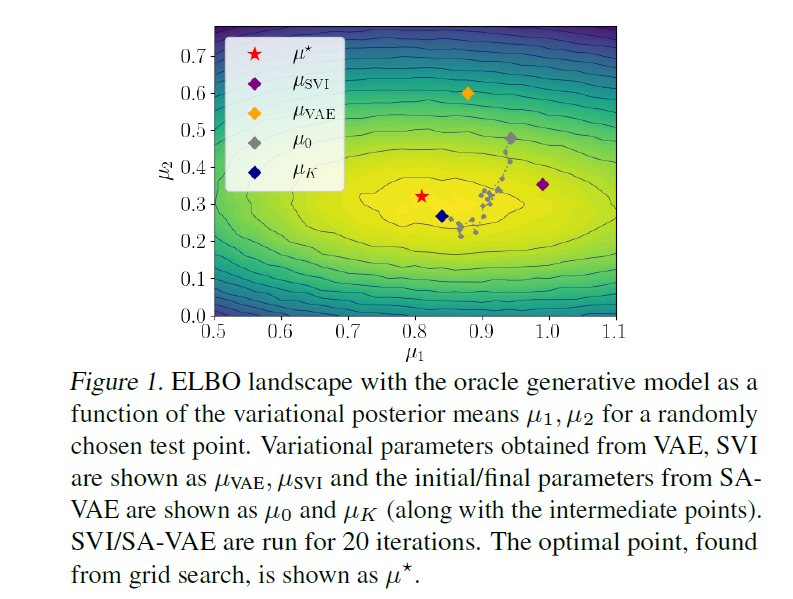
\includegraphics[width=0.8\textwidth]{figure6.png}
\label{fig1}
\end{figure}

\end{frame}



\begin{frame}{Experiments}

\begin{figure}[t]
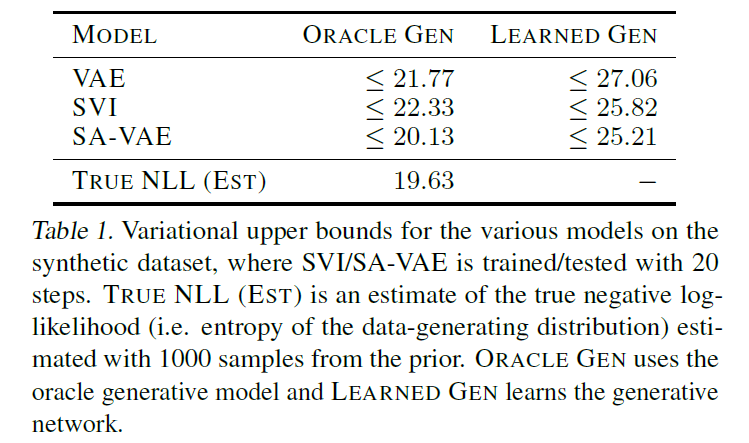
\includegraphics[width=0.8\textwidth]{figure7.png}
\label{fig1}
\end{figure}

\end{frame}



\begin{frame}{Experiments}

\begin{figure}[t]
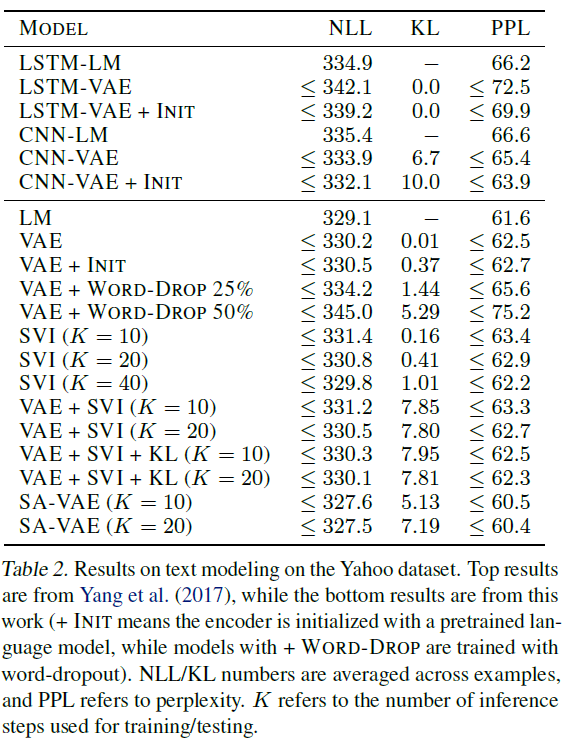
\includegraphics[width=0.5\textwidth]{figure8.png}
\label{fig1}
\end{figure}

\end{frame}



\begin{frame}{Experiments}

\begin{figure}[t]
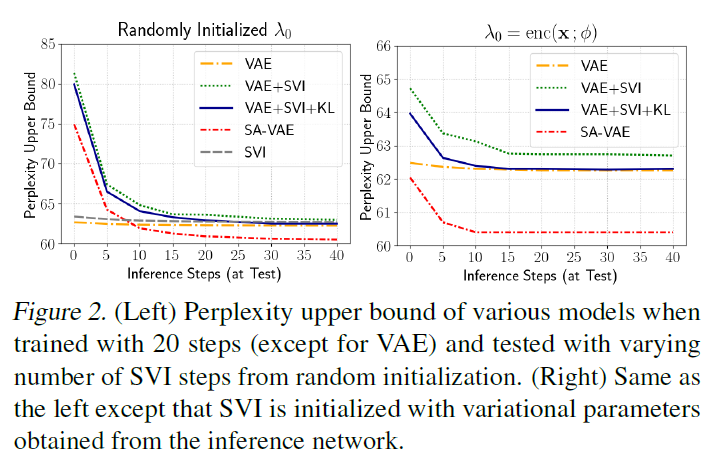
\includegraphics[width=0.8\textwidth]{figure9.png}
\label{fig1}
\end{figure}

\end{frame}



\title[Iterative Amortized Inference]{Iterative Amortized Inference}

\author[Joseph Marino, Yisong Yue and Stephan Mandt]{Joseph Marino, Yisong Yue and Stephan Mandt\\  presenter: Shen Yuan} % Insert your name

\begin{frame}	

\titlepage
	
\end{frame}	



\begin{frame}[noframenumbering]
\begin{itemize}
    \begin{LARGE}
    \item Iterative Amortized Inference
    \item \light{Iterative Inference in Latent Gaussian Models}
    \item \light{Experiments}
    \end{LARGE}
\end{itemize}
\end{frame}



\begin{frame}{Iterative Amortized Inference}

\begin{figure}[t]
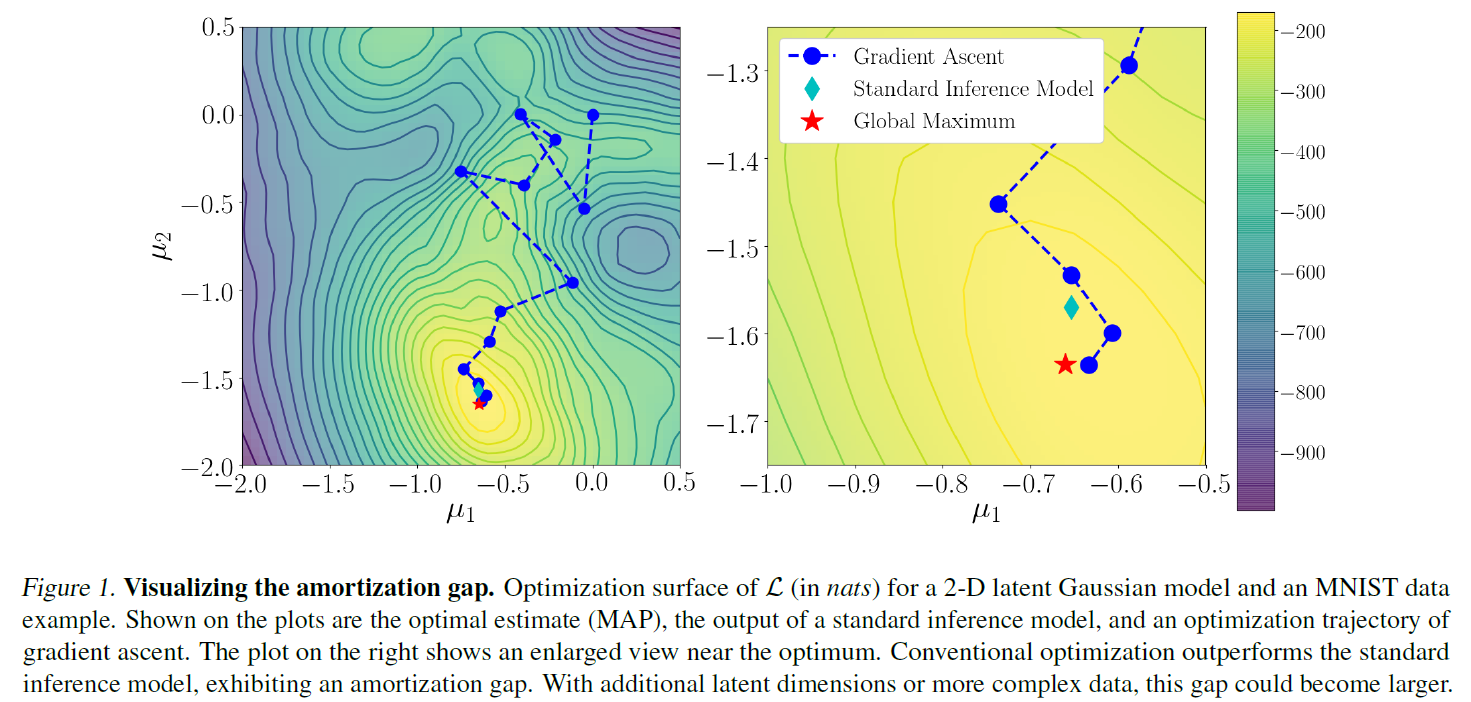
\includegraphics[width=0.95\textwidth]{figure11.png}
\label{fig1}
\end{figure}

\end{frame}



\begin{frame}{Iterative Amortized Inference}

We denote the iterative inference model as $f$ with parameters $\phi$.

\begin{eqnarray*}
\begin{aligned}
\bm{\lambda}_{t+1}^{(i)} \gets f_t(\nabla_{\bm{\lambda}} \mathcal{L}_t^{(i)}, \bm{\lambda}_t^{(i)}; \phi)
\end{aligned}    
\end{eqnarray*}

where $\bm{\lambda}$ is the distribution parameters of $q(\bm{z}|\bm{x})$, $\mathcal{L}_t^{(i)} \equiv \mathcal{L}(\bm{x}^{(i)}, \bm{\lambda}_t^{(i)}; \phi)$ represents the ELBO for data example $\bm{x}^{(i)}$ at inference iteration $t$.

\end{frame}



\begin{frame}{Iterative Amortized Inference}

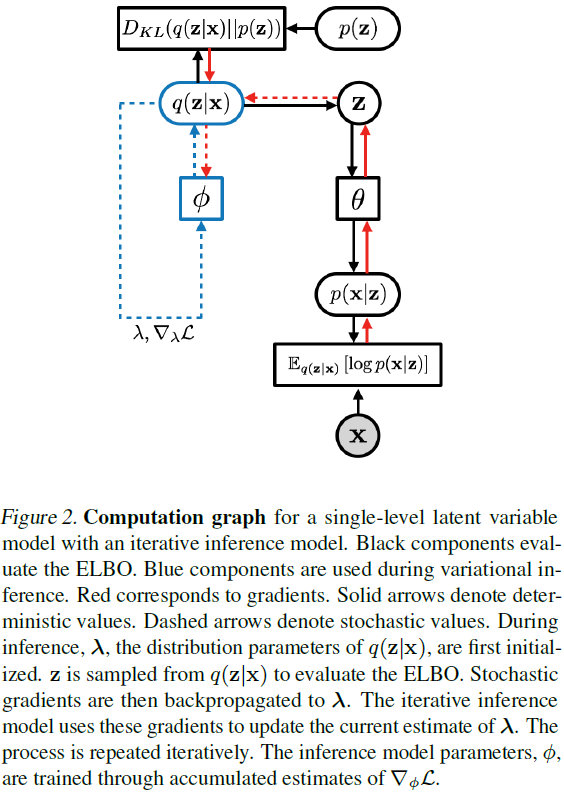
\includegraphics[width=0.45\textwidth,align=c]{figure12.png}
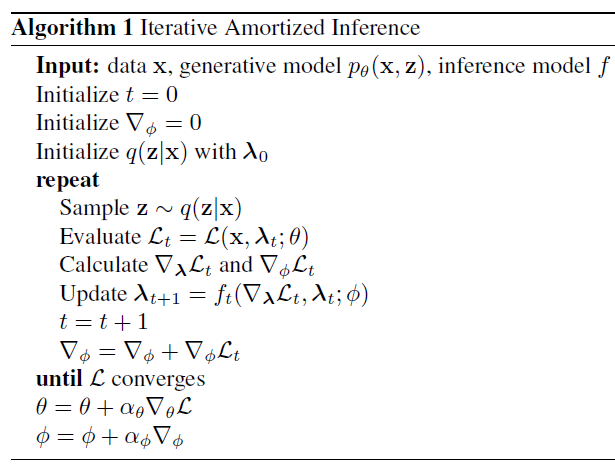
\includegraphics[width=0.45\textwidth,align=c]{figure18.png}
% 't' align top, 'c' align middle, '' align bottom

\end{frame}



\begin{frame}{Semi-Amortized Variational Autoencoders}

\begin{figure}[H]
\centering
\subfigure{
\label{Fig.sub.11}
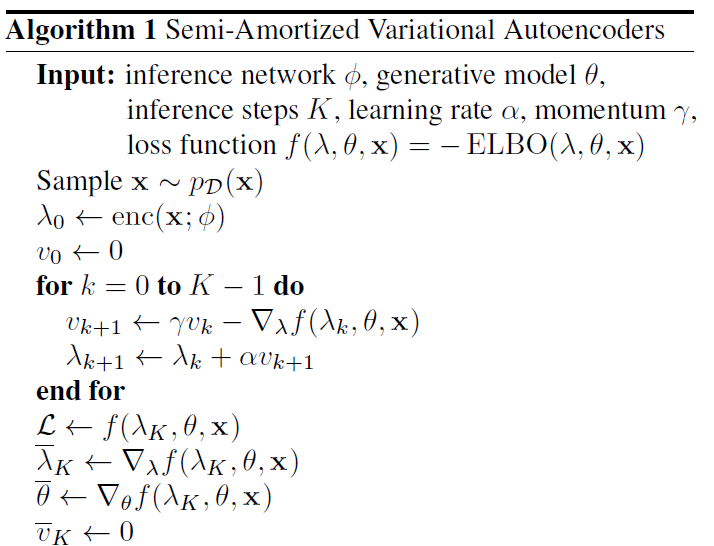
\includegraphics[width=0.45\textwidth]{figure4.png}}
\subfigure{
\label{Fig.sub.12}
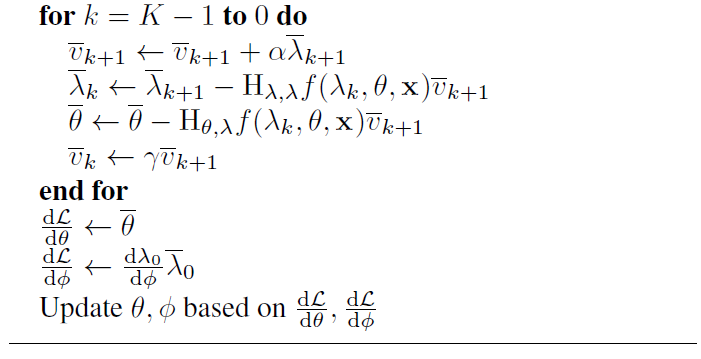
\includegraphics[width=0.45\textwidth]{figure5.png}}
\label{fig1}
\end{figure}

\end{frame}



\begin{frame}[noframenumbering]
\begin{itemize}
    \begin{LARGE}
    \item \light{Iterative Amortized Inference}
    \item Iterative Inference in Latent Gaussian Models
    \item \light{Experiments}
    \end{LARGE}
\end{itemize}
\end{frame}



\begin{frame}{Iterative Inference in Latent Gaussian Models}

We now describe an instantiation of iterative inference models for (single-level) latent Gaussian models, which have a Gaussian prior density over latent variables: $p(\bm{z})=\mathcal{N}(\bm{z};\bm{\mu}_p, \text{diag} \, \bm{\sigma}^2_p)$

~\\
While the approximate posterior is also chosen as Gaussian:$q(\bm{z}|\bm{x})=\mathcal{N}(\bm{z};\bm{\mu}_q,\text{diag}\, \bm{\sigma}^2_q)$


\begin{eqnarray*}
\begin{aligned}
&\bm{\mu}_{q,t+1}=f_t^{\bm{\mu}_q}(\nabla_{\bm{\mu}_q} \mathcal{L}_t, \bm{\mu}_{q,t}; \phi),\\
&\bm{\sigma}_{q,t+1}^2=f_t^{\bm{\sigma}^2_q}(\nabla_{\bm{\sigma}_q^2} \mathcal{L}_t, \bm{\sigma}^2_{q,t}; \phi)
\end{aligned}    
\end{eqnarray*}

where $f_t^{\bm{\mu}_q}$ and $f_t^{\bm{\sigma}^2_q}$ are the iterative inference models for
updating $\bm{\mu}_q$ and $\bm{\sigma}_q^2$ respectively.

\end{frame}



\begin{frame}{Iterative Inference in Latent Gaussian Models}

For instance, assuming a Gaussian output density $q(\bm{x}|\bm{z})=\mathcal{N}(\bm{x};\bm{\mu}_{\bm{x}},\text{diag}\, \bm{\sigma}^2_{\bm{x}})$, the gradient for $\bm{\mu}_q$ is

\begin{eqnarray*}
\begin{aligned}
\nabla_{\bm{\mu}_q} \mathcal{L} = \bm{J}^\top \varepsilon_{\bm{x}} - \varepsilon_{\bm{z}}
\end{aligned}    
\end{eqnarray*}

where the Jacobian ($\bm{J}$), bottom-up errors ($\varepsilon_{\bm{x}}$), and top-down errors ($\varepsilon_{\bm{z}}$) are defined as

\begin{eqnarray*}
\begin{aligned}
\bm{J} &\equiv \E_{\bm{z} \sim q(\bm{z}|\bm{x})}[\frac{\partial \bm{\mu_x}}{\partial \bm{\mu_q}}]\\
\varepsilon_{\bm{x}} &\equiv  \E_{\bm{z} \sim q(\bm{z}|\bm{x})}[(\bm{x}-\bm{\mu_x}) / \bm{\sigma}_{\bm{x}}^2]\\
\varepsilon_{\bm{z}} &\equiv  \E_{\bm{z} \sim q(\bm{z}|\bm{x})}[(\bm{z}-\bm{\mu_p}) / \bm{\sigma}_{\bm{p}}^2]
\end{aligned}    
\end{eqnarray*}

\end{frame}



\begin{frame}{Iterative Inference in Latent Gaussian Models}

\begin{eqnarray*}
\begin{aligned}
\varepsilon_{\bm{x}} &= \bm{Ax+b}\\
\bm{A} &\equiv \E_{q(\bm{z}|\bm{x})}[(\text{diag}\, \bm{\sigma}^2_{\bm{x}})^{-1}]\\
\bm{b} &\equiv -\E_{q(\bm{z}|\bm{x})}[\frac{\bm{\mu_x}}{\bm{\sigma}^2_{\bm{x}}}]
\end{aligned}    
\end{eqnarray*}

Assuming that the initial approximate posterior and prior are both constant, then in expectation, $\bm{A}$, $\bm{b}$, and $\varepsilon_{\bm{z}}$ are constant across all data examples at the first inference iteration. \\
Using proper weight initialization and input normalization, it is equivalent to input $\bm{x}$ or an affine transformation of $\bm{x}$ into a fully-connected neural network.\\
Therefore, standard inference models are equivalent to the special case of a one-step iterative inference model.

\end{frame}



\begin{frame}[noframenumbering]
\begin{itemize}
    \begin{LARGE}
    \item \light{Iterative Amortized Inference}
    \item \light{Iterative Inference in Latent Gaussian Models}
    \item Experiments
    \end{LARGE}
\end{itemize}
\end{frame}



\begin{frame}{Experiments}

\begin{figure}[t]
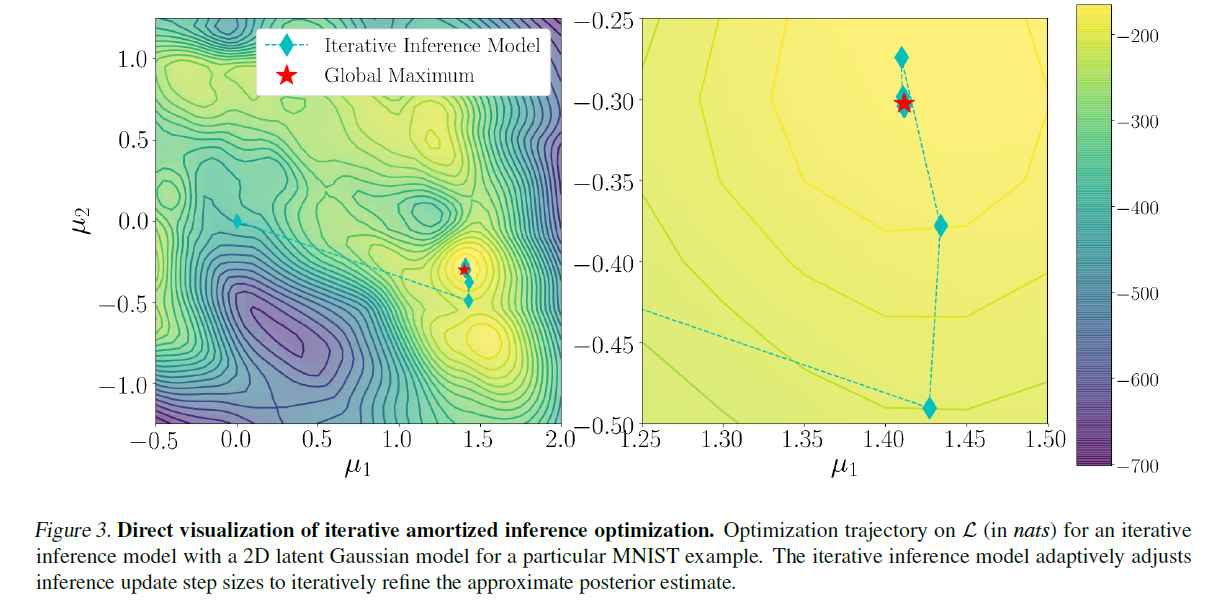
\includegraphics[width=0.9\textwidth]{figure13.png}
\label{fig1}
\end{figure}

\end{frame}



\begin{frame}{Experiments}


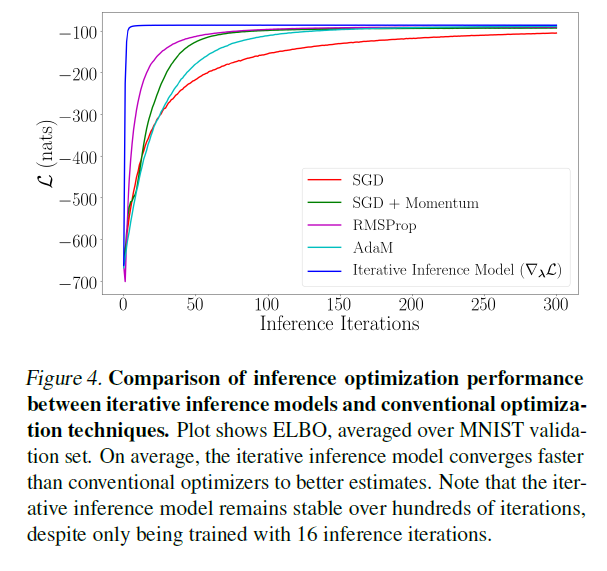
\includegraphics[width=0.48\textwidth, align=c]{figure14.png}
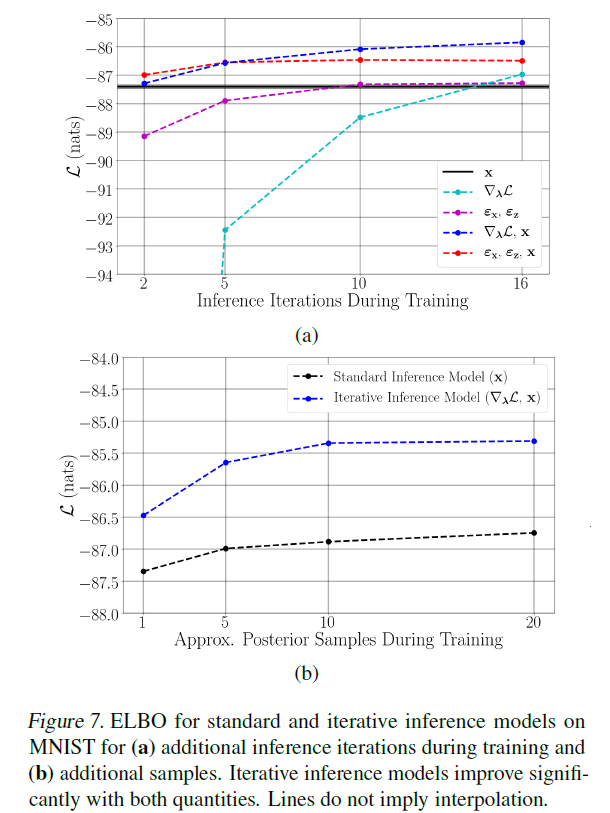
\includegraphics[width=0.48\textwidth, align=c]{figure15.png}

\end{frame}



\end{document}	% Done!

